\documentclass[onecolumn,conference]{IEEEtran}
\IEEEoverridecommandlockouts
% The preceding line is only needed to identify funding in the first footnote. If that is unneeded, please comment it out.
\usepackage{cite}
\usepackage{amsmath,amssymb,amsfonts}
\usepackage{algorithmic}
\usepackage{graphicx}
\usepackage{textcomp}
\usepackage{xcolor}
\usepackage[linktocpage=true,colorlinks,citecolor=blue,pagebackref=true]{hyperref}
\usepackage{datetime}

\def\BibTeX{{\rm B\kern-.05em{\sc i\kern-.025em b}\kern-.08em
T\kern-.1667em\lower.7ex\hbox{E}\kern-.125emX}}

\begin{document}

    \title{Effect of Buffer Size and Packet Delay on the Survivability of Packet Switched Networks}
    \IEEEpubid{$1^{st}$ National Conference on New Approaches in Computer Engineering and Information Retrieval, 7 October 2013}
    \date{7 October 2013}
    \author{\IEEEauthorblockN{1\textsuperscript{st} Vahid Mavaji}
    \IEEEauthorblockA{\textit{Department of Computer Engineering} \\
    \textit{Sharif University of Technology}\\
    Tehran, Iran \\
    mavaji@alum.sharif.edu}
    \and
    \IEEEauthorblockN{2\textsuperscript{nd} Bahareh Abbasi}
    \IEEEauthorblockA{\textit{Department of Computer Engineering} \\
    \textit{Sharif University of Technology}\\
    Tehran, Iran \\
    b\_abbasi@alum.sharif.edu}
    }

    \maketitle

    \begin{abstract}
        In this paper, the survivability of general-case packet-switched networks is studied. Most of network properties are considered as random variables and a queuing-theory based model is derived. In this model, the effect of buffer size and packets' delay on the survivability of the network is considered. Simulation results are used to validate the proposed model. The simulation results agree very well with the model.
    \end{abstract}

    \begin{IEEEkeywords}
        Survivability, Packet Switched Networks, Buffer Size, Delay
    \end{IEEEkeywords}

    \section{Introduction} \label{sec:intro}
    The problem of designing networks able to survive an enemy attack or natural disaster is of paramount importance. Recent work has focused on the mathematical formulation of physically meaningful survivability criteria, the development of analysis methods to rank networks in terms of these criteria, and the generation of networks which are optimal with respect to these criteria. Numerous partial results for a variety of network models are available.

    The study of network survivability has been divided into two nearly disjoint areas: deterministic survivability and probabilistic survivability. In the former, an adversary is usually assumed to have complete knowledge about the system to be attacked and also uses a deterministic attack strategy. In a probabilistic model, the adversary may have only partial information about the enemy's network or may employ a randomized attack strategy.

    Because of the dichotomy of network and attack models, typical survivability criteria can also be classified as either deterministic or probabilistic. A network may be considered to ``survive'' an attack if 1) all points (nodes) can communicate with each other; 2) there are some flow paths between specified pairs of points; 3) the number of points in the largest connected section exceeds a specified threshold; or 4) the shortest surviving path between each pair of points is no longer than a specified length.

    The object of a deterministic analysis might be to determine if these criteria are met subject to a known attack while a probabilistic analysis might seek to find the probabilities that these criteria will be satisfied. Corresponding design objectives could then be constructing networks subject to fixed resources which maximize the effort the adversary must make to ``destroy'' the network, or the probability that the network will survive.

    The purpose of this paper is to perform a probabilistic analysis of packet-switched network considering the packet loss and delay of packets as survivability measures. The effect of buffer size is also examined.

    The rest of this paper is organized as follows: in Section \ref{sec:rlwork} a literature survey is presented. In Section \ref{sec:prel} the preliminaries and assumption of the problem are clarified. In Section \ref{sec:eval} a model for evaluating the survivability is derived. Section~\ref{sec:simres} presents the simulation results and Section \ref{sec:conc} concludes the paper.

    \section{Related Work} \label{sec:rlwork}
    Four of the issues that arise in the development of survivable architectures are discussed in \cite{b5}. A framework for providing survivability to group communications, where part of the underlying traffic layer infrastructure is connection oriented, is presented in \cite{b13}. The framework is multi-layered to express the virtual overlays inherent to networked systems.

    In \cite{b14}, the use of a hop-limit constraint with techniques to provide survivability for connection-oriented ATM group communications is examined. A hop-limit: (1) limits the number of routes considered such that the routing problems of higher order complexity can be solved, and (2) limits the length of any individual route to meet specific Quality of Service guarantees (such as delay).

    A quantitative approach to evaluate network survivability is proposed in \cite{b2}. The network survivability is perceived as a composite measure consisting of both network failure duration and failure impact on the network. A wireless ad-hoc network is analyzed as an example, and the excess packet loss due to failures (ELF) is taken as the survivability performance measure. To obtain ELF, a two-phase approach is adopted consisting of the steady-state availability analysis and system transient performance analysis. Assuming Markovian property for the system, this measure is obtained by solving a set of Markov models.

    In \cite{b11}, a mathematical model for an efficient lightpath routing called \textit{Load Distribution-Survivable Lightpath Routing (LD-SLR)} is proposed, which can mitigate the impact of the failure disruption in the OVPN by introducing the load distribution concept to the survivable lightpath routing.

    In \cite{b12}, the following question is addressed: what is the minimum number of links that has to be added to a physical topology so that the survivable routing of a logical ring is possible? An ILP formulation for finding the optimal solution of the problem is provided. An optimization model for the design of survivable wireless access networks is proposed in \cite{b1}. The main objective of the model is to optimize the network design cost of wireless backhaul networks while meeting survivability requirements. A simple and efficient heuristic method to solve the network design model for large network problem sizes within a reasonable computational time is also presented.

    Several survivable architectures for telephone subscriber network based on common survivability principles are proposed in \cite{b6}. In order to quantitatively assess the effectiveness of design alternatives, a set of analytical models are developed to derive various survivability measures. In \cite{b7}, a general survivability quantification framework which is applicable to a wide range of system architectures, applications, failure/recovery behaviors, and desired metrics is proposed. An illustrative example of a telecommunications switching system is given for the ease of discussion.

    A composite model for survivability that consists of performance and availability analysis is proposed in \cite{b3}. An analytical technique is presented to find the excess loss due to failure (ELF) when the system is operating in gracefully degraded states.

    In \cite{b8}, the Spare Capacity Allocation (SCA) problem structure is unraveled using a matrix-based model. A fast and efficient approximation algorithm, termed successive survivable routing (SSR), is also developed. The problem of provisioning spare capacity in multi-layer backbone networks in order to meet survivability requirements is considered in \cite{b9}. A matrix based model is presented showing how failure propagation can be mapped across network layers.

    In \cite{b10} authors propose a survivability scheme to support reliable service of the wireless access point level (BS-base station system). With the survivability scheme, the mobile network can use an overlap BS of the cellular network architecture after a BS system failure. The performance of the proposed scheme is analyzed using Markov models. The proposed scheme shows that service of the mobile network can be provided under the BS system failure.

    Through analyzing the changes of key services' performance index value before and after evaluation, \cite{b15} proposed a novel quantitative analysis method for network survivability based on grey relational analysis. Starting with the normalization of decision matrix with interval number, the proposed method firstly applies grey relational analysis to assess the best affiliate degree and survival probability of every key service. Then, it analyzes the changes of every key service's survivability based on network entropy difference. Finally, it obtains the synthetic analysis for the whole network survivability.

    \section{Preliminaries} \label{sec:prel}
    For evaluating the survivability of packet switched networks, we suppose that each of network nodes has the structure depicted in Fig. \ref{fig:1}, i.e. each of them is an $m/m/1/k$ queue.

    \begin{figure}[htbp]
        \centering
        \makebox[\textwidth]{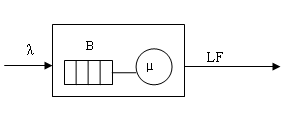
\includegraphics{rbpj1.png}}
        \caption{Structure of network nodes}
        \label{fig:1}
    \end{figure}

    Moreover, suppose that the network is a set of such nodes, so that its topology is unknown. A sample network is shown in Fig. \ref{fig:2}.

    \begin{figure}[htbp]
        \centering
        \makebox[\textwidth]{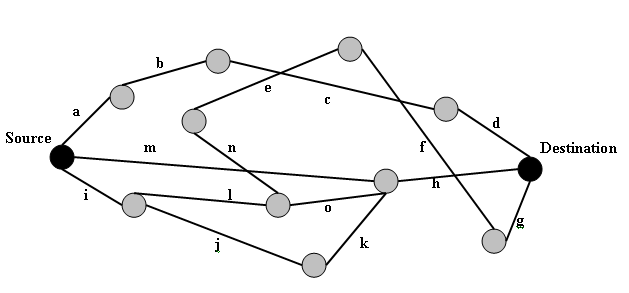
\includegraphics{rbpj2.png}}
        \caption{A sample network consisting of $m/m/1/k$ nodes}
        \label{fig:2}
    \end{figure}

    For example, there are several potential paths between the source and the destination nodes. Suppose that the path $\{a, b, c, d\}$ is established. If for some reason, this path is disconnected, another path can be used as a replacement. For instance, if link c fails, the paths $\{m, h\}$ or $\{i, l, o, h\}$ can be used.

    An important consideration is that in general case and in packet switched network, the network topology in unknown. That is, we have to consider anything as statistical. For performing mathematical operations, most of network parameters most be treated as random variables. The following assumptions about nodes and the network itself are made:

    \begin{enumerate}
        \item Network nodes have the same statistical properties.
        \item The routing algorithm selects each of alternative paths with equal probability.
        \item The network links fail independently from each other.
        \item If at least one of the path's links fails, we consider that path as failed (disconnected).
        \item The network paths have the same statistical properties.
        \item The number of nodes of a path is a random variable called $N$.
        \item The failure probability of each link is $LF$.
        \item The buffer size of each node is equal to $B$.
        \item Packet arrival to each node has the Poisson distribution with parameter $\lambda$.
        \item Service rate to the packets is $\mu$.
        \item Initially, there are $R$ paths.
    \end{enumerate}

    \section{Evaluating the Survivability} \label{sec:eval}
    With the above assumptions, we begin the modeling process.

    \textbf{Step 1:} we calculate the packet loss of a typical path. The packet loss of a path, $PL_{path}$, is the sum of packet losses of all of its constituent nodes:
    \begin{equation}
        PL_{path}=\sum_{i=1}^nPL_i
    \end{equation}
    Now, we obtain the expectation or mean value of packet loss in a path. The long term average rate of packet loss in a node is equal to packet loss probability of that node, denoted it by $PL_i$.

    \begin{equation}
        E\left[PL_{path}\right]=E\left[\sum_{i=1}^nPL_i\right]=\sum_{i=1}^{E\left[n\right]}E\left[PL_i\right]
    \end{equation}

    Now, we have to calculate the mean value of packet loss in each node. The packet loss probability is the probability that the buffer is full and there is no space for new packets. From queuing theory it is equal to PL \cite{b4}:

    \begin{equation}
        PL=P_{B+1}=\frac{{\left(\frac{\lambda}{\mu}\right)^{B+1}}{\left(1-\frac{\lambda}{\mu}\right)} }
        {{1-\left(\frac{\lambda}{\mu}\right)}^{B+2}}
    \end{equation}

    An important thing to consider is that our model is of open queuing network type and the assumption of independence of arrival is no longer held. That is, the arrival rate to the second node is dependent on service rate and packet loss of the first node. In the same manner, the third node is dependent on the second node and so on. Therefore the Poisson property of arrivals in no longer valid and the computation will be very complex. For this reason, we define an approximating assumption: the arrival rate of all nodes remain Poisson, but the corresponding $\lambda$ changes. For example, suppose that we want to know the arrival rate of node i; we know that the arrival rate of its preceding node is $\lambda_{i-1}$ and the packets are lost with the probability $PL_{i-1}$. Therefore, with a simple approximation, the arrival rate of the $i^{th}$ node can be calculated:

    \begin{equation}
        \lambda_i=\lambda_{i-1} \times PL_{i-1}
    \end{equation}
    And also:
    \begin{equation}
        \lambda_1=\lambda
    \end{equation}

    \textbf{Step 2:} we calculate the mean value of a typical path's delay. A packet traversing from source to destination, wait a time equal to $W$ in each node, then enters a link and has a propagation delay equal to $t_p$. Therefore, as there are $N$ nodes and $N-1$ links, the path's delay is:
    \begin{equation}
        Delay_{path}=\sum_{i=1}^{E\left[n\right]}W_i+\left(N-1\right)t_p
    \end{equation}

    Where, $W_i$ is the value of $W$ when $\lambda=\lambda_i$, and $W$ is the waiting time of a $m/m/1/k$ queue which in turn is \cite{b4}

    \begin{equation}
        W=\sum_{n=0}^B\frac{\left(n+1\right)P_n}
        {\mu\left(1-P_{B+1}\right)}=\frac{L-\left(B+2\right)P_{B+1}+1}{\mu\left(1-P_{B+1}\right)}
    \end{equation}

    $L$ is the mean number of packets in a node and is equal to \cite{b4}:

    \begin{equation}
        L=\frac{\lambda\left(1+\left(B+1\right)\left(\frac{\lambda}{\mu}\right)^{B+2}-\left(B+2\right)\left(\frac{\lambda}{\mu}\right)^{B+1}\right)}{\left(\mu-\lambda\right)\left(1-\left(\frac{\lambda}{\mu}\right)^{B+2}\right)}
    \end{equation}

    Therefore, we have:

    \begin{equation}
        \begin{split}
            &E\left[Delay_{path}\right]\\&=\sum_{i=1}^n\left(\frac{L_i-\left(B+2\right)P_{i,B+1}+1}{\mu\left(1-P_{i,B+1}\right)}\right)+\left(E\left[N\right]-1\right)E\left[t_p\right]=\sum_{i=1}^n\left(\frac{L_i-\left(B+2\right)P_{i,B+1}+1}{\mu\left(1-P_{i,B+1}\right)}\right)+\frac{E\left[Len_{link}\right]}{C}
        \end{split}
    \end{equation}

    $Len_{link}$ is a random variable and demonstrates the distribution of links' length. $C$ is the light speed or more precisely, the propagation speed of waves in the links.

    Now, for evaluating the survivability of a path, we employ the following reasoning:
    If the path doesn't fail, as long as the values of packet loss and packets' delay don't exceed a specific threshold, the survivability is equal to one. When these values exceed their thresholds, the value of survivability has inverse relation with the difference of packet loss and delay to their threshold. Now, if this path fails, with some probability, a spare path is chosen, and then the survivability of this new path determines the survivability of the previous one. Therefore the similarity of the statistical properties of the paths helps us and the following equations are obtained:

    \begin{equation}
        \begin{split}
            &Survivability\\&=\frac{1-P_{path\_failure}}{1+\max\left(PL_{path}-T_{PL},0\right)+\max\left(Delay_{path}-T_{Delay},0\right)}+P_{path\_failure}\times P_{existence\_of\_backup\_path}\times
            Survivability
        \end{split}
    \end{equation}

    \begin{equation}
        \begin{split}
            &\Rightarrow Survivability
            \\&=\frac{\left( 1-P_{path\_failure} \right)}
            {\left(
            \left(1+\max\left(PL_{path}-T_{PL},0\right)+\max\left(Delay_{path}-T_{Delay},0 \right)\right)
            \times
            \left(1- P_{path\_failure}\times P_{existence\_of\_backup\_path} \right)
            \right)}
        \end{split}
    \end{equation}

    $P_{path\_failure}$ is the failure probability of the path and its value is equal to the probability that at least, one of the path's links fails. Therefore:

    \begin{equation}
        P_{path\_failure}=1-\left( 1-LF \right)^{E\left[ N \right]-1}
    \end{equation}

    $P_{existence\_of\_backup\_path}$, is the probability of existence of a spare path. Considering the fact that initially, there are $R$ non-failed paths and the probability of non-existence of any spare path is equal to the probability that $R-1$ paths fail, we have:

    \begin{equation}
        P_{existence\_of\_backup\_path} = 1-\left( P_{path\_failure} \right)^{R-1}
    \end{equation}

    $T_{PL}$ and $T_{Delay}$ are the threshold values for packet loss and packets' delay respectively. That is, if these parameters exceed the thresholds, survivability begins to decrease with inverse relation.

    The value of survivability is between zero and one. Proof:

    \begin{equation}
        \begin{split}
            Let:&P_1=P_{path\_failure},\\
            &P_2=P_{existence\_of\_backup\_path} \\
            &0 \leq P_1 \leq 1, \\
            &0 \leq P_2 \leq 1 \\
            &\Rightarrow P_1 \geq P_1P_2
        \end{split}
    \end{equation}

    \begin{equation}
        \begin{split}
            &\Rightarrow 1-P_1\leq 1-P_1P_2 \\
            &\Rightarrow \frac{1-P_1}{1-P_1P_2}\leq1
        \end{split}
    \end{equation}

    \begin{equation}
        \begin{split}
            & 1+\max\left( PL_{path} -T_{PL},0 \right)+\max\left( Delay_{path}-T_{Delay},0 \right) \geq 1 \\
            \Rightarrow & \frac{1}{1+\max\left( PL_{path} -T_{PL},0 \right)+\max\left( Delay_{path}-T_{Delay},0 \right)} \leq 1 \\
            \Rightarrow & \frac{1-P_1}{1-P_1P_2}\times\frac{1}{1+\max\left( PL_{path} -T_{PL},0 \right)+\max\left( Delay_{path}-T_{Delay},0 \right)}\leq 1 \\
            \Rightarrow & Survivability \leq 1
        \end{split}
    \end{equation}

    It is easy to show that the value of survivability is always greater or equal to zero, so:
    \begin{equation}
        0 \leq Survivability \leq 1
    \end{equation}
    
    \section{Simulation Results} \label{sec:simres}

    \section{Conclusion} \label{sec:conc}
    We have presented in this paper a queuing-theory based model for general-case packet-switched network in which the nodes are $m/m/1/k$ queues. Parameters such as buffer size and packets' delay were considered important in determining the survivability of such network. Simulation results are in accordance with the model. It was shown that increasing the buffer size has a positive impact on the survivability. Increasing the number of nodes and the link failure probability both decrease the survivability.

    The future work is to impose more realistic limitations on network properties such as dependence of node failures on each other, the impact of traffic resulted from path replacement on packet loss, the impact of link failure on packets' delay, assuming different structures for network nodes, dependence of link failures on each other, the possibility of repair and recovery in the network and so on.
    %    \section{Ease of Use}
    %
    %    \subsection{Maintaining the Integrity of the Specifications}
    %
    %    The IEEEtran class file is used to format your paper and style the text. All margins,
    %    column widths, line spaces, and text fonts are prescribed; please do not
    %    alter them. You may note peculiarities. For example, the head margin
    %    measures proportionately more than is customary. This measurement
    %    and others are deliberate, using specifications that anticipate your paper
    %    as one part of the entire proceedings, and not as an independent document.
    %    Please do not revise any of the current designations.
    %
    %    \section{Prepare Your Paper Before Styling}
    %    Before you begin to format your paper, first write and save the content as a
    %    separate text file. Complete all content and organizational editing before
    %    formatting. Please note sections \ref{AA}--\ref{SCM} below for more information on
    %    proofreading, spelling and grammar.
    %
    %    Keep your text and graphic files separate until after the text has been
    %    formatted and styled. Do not number text heads---{\LaTeX} will do that
    %    for you.
    %
    %    \subsection{Abbreviations and Acronyms}\label{AA}
    %    Define abbreviations and acronyms the first time they are used in the text,
    %    even after they have been defined in the abstract. Abbreviations such as
    %    IEEE, SI, MKS, CGS, ac, dc, and rms do not have to be defined. Do not use
    %    abbreviations in the title or heads unless they are unavoidable.
    %
    %    \subsection{Units}
    %    \begin{itemize}
    %        \item Use either SI (MKS) or CGS as primary units. (SI units are encouraged.) English units may be used as secondary units (in parentheses). An exception would be the use of English units as identifiers in trade, such as ``3.5-inch disk drive''.
    %        \item Avoid combining SI and CGS units, such as current in amperes and magnetic field in oersteds. This often leads to confusion because equations do not balance dimensionally. If you must use mixed units, clearly state the units for each quantity that you use in an equation.
    %        \item Do not mix complete spellings and abbreviations of units: ``Wb/m\textsuperscript{2}'' or ``webers per square meter'', not ``webers/m\textsuperscript{2}''. Spell out units when they appear in text: ``. . . a few henries'', not ``. . . a few H''.
    %        \item Use a zero before decimal points: ``0.25'', not ``.25''. Use ``cm\textsuperscript{3}'', not ``cc''.)
    %    \end{itemize}
    %
    %    \subsection{Equations}
    %    Number equations consecutively. To make your
    %    equations more compact, you may use the solidus (~/~), the exp function, or
    %    appropriate exponents. Italicize Roman symbols for quantities and variables,
    %    but not Greek symbols. Use a long dash rather than a hyphen for a minus
    %    sign. Punctuate equations with commas or periods when they are part of a
    %    sentence, as in:
    %    \begin{equation}
    %        a+b=\gamma\label{eq}
    %    \end{equation}
    %
    %    Be sure that the
    %    symbols in your equation have been defined before or immediately following
    %    the equation. Use ``\eqref{eq}'', not ``Eq.~\eqref{eq}'' or ``equation \eqref{eq}'', except at
    %    the beginning of a sentence: ``Equation \eqref{eq} is . . .''
    %
    %    \subsection{\LaTeX-Specific Advice}
    %
    %    Please use ``soft'' (e.g., \verb|\eqref{Eq}|) cross references instead
    %    of ``hard'' references (e.g., \verb|(1)|). That will make it possible
    %    to combine sections, add equations, or change the order of figures or
    %    citations without having to go through the file line by line.
    %
    %    Please don't use the \verb|{eqnarray}| equation environment. Use
    %    \verb|{align}| or \verb|{IEEEeqnarray}| instead. The \verb|{eqnarray}|
    %    environment leaves unsightly spaces around relation symbols.
    %
    %    Please note that the \verb|{subequations}| environment in {\LaTeX}
    %    will increment the main equation counter even when there are no
    %    equation numbers displayed. If you forget that, you might write an
    %    article in which the equation numbers skip from (17) to (20), causing
    %    the copy editors to wonder if you've discovered a new method of
    %    counting.
    %
    %    {\BibTeX} does not work by magic. It doesn't get the bibliographic
    %    data from thin air but from .bib files. If you use {\BibTeX} to produce a
    %    bibliography you must send the .bib files.
    %
    %    {\LaTeX} can't read your mind. If you assign the same label to a
    %    subsubsection and a table, you might find that Table I has been cross
    %    referenced as Table IV-B3.
    %
    %    {\LaTeX} does not have precognitive abilities. If you put a
    %    \verb|\label| command before the command that updates the counter it's
    %    supposed to be using, the label will pick up the last counter to be
    %    cross referenced instead. In particular, a \verb|\label| command
    %    should not go before the caption of a figure or a table.
    %
    %    Do not use \verb|\nonumber| inside the \verb|{array}| environment. It
    %    will not stop equation numbers inside \verb|{array}| (there won't be
    %    any anyway) and it might stop a wanted equation number in the
    %    surrounding equation.
    %
    %    \subsection{Some Common Mistakes}\label{SCM}
    %    \begin{itemize}
    %        \item The word ``data'' is plural, not singular.
    %        \item The subscript for the permeability of vacuum $\mu_{0}$, and other common scientific constants, is zero with subscript formatting, not a lowercase letter ``o''.
    %        \item In American English, commas, semicolons, periods, question and exclamation marks are located within quotation marks only when a complete thought or name is cited, such as a title or full quotation. When quotation marks are used, instead of a bold or italic typeface, to highlight a word or phrase, punctuation should appear outside of the quotation marks. A parenthetical phrase or statement at the end of a sentence is punctuated outside of the closing parenthesis (like this). (A parenthetical sentence is punctuated within the parentheses.)
    %        \item A graph within a graph is an ``inset'', not an ``insert''. The word alternatively is preferred to the word ``alternately'' (unless you really mean something that alternates).
    %        \item Do not use the word ``essentially'' to mean ``approximately'' or ``effectively''.
    %        \item In your paper title, if the words ``that uses'' can accurately replace the word ``using'', capitalize the ``u''; if not, keep using lower-cased.
    %        \item Be aware of the different meanings of the homophones ``affect'' and ``effect'', ``complement'' and ``compliment'', ``discreet'' and ``discrete'', ``principal'' and ``principle''.
    %        \item Do not confuse ``imply'' and ``infer''.
    %        \item The prefix ``non'' is not a word; it should be joined to the word it modifies, usually without a hyphen.
    %        \item There is no period after the ``et'' in the Latin abbreviation ``et al.''.
    %        \item The abbreviation ``i.e.'' means ``that is'', and the abbreviation ``e.g.'' means ``for example''.
    %    \end{itemize}
    %    An excellent style manual for science writers is \cite{b7}.
    %
    %    \subsection{Authors and Affiliations}
    %    \textbf{The class file is designed for, but not limited to, six authors.} A
    %    minimum of one author is required for all conference articles. Author names
    %    should be listed starting from left to right and then moving down to the
    %    next line. This is the author sequence that will be used in future citations
    %    and by indexing services. Names should not be listed in columns nor group by
    %    affiliation. Please keep your affiliations as succinct as possible (for
    %    example, do not differentiate among departments of the same organization).
    %
    %    \subsection{Identify the Headings}
    %    Headings, or heads, are organizational devices that guide the reader through
    %    your paper. There are two types: component heads and text heads.
    %
    %    Component heads identify the different components of your paper and are not
    %    topically subordinate to each other. Examples include Acknowledgments and
    %    References and, for these, the correct style to use is ``Heading 5''. Use
    %    ``figure caption'' for your Figure captions, and ``table head'' for your
    %    table title. Run-in heads, such as ``Abstract'', will require you to apply a
    %    style (in this case, italic) in addition to the style provided by the drop
    %    down menu to differentiate the head from the text.
    %
    %    Text heads organize the topics on a relational, hierarchical basis. For
    %    example, the paper title is the primary text head because all subsequent
    %    material relates and elaborates on this one topic. If there are two or more
    %    sub-topics, the next level head (uppercase Roman numerals) should be used
    %    and, conversely, if there are not at least two sub-topics, then no subheads
    %    should be introduced.
    %
    %    \subsection{Figures and Tables}
    %    \paragraph{Positioning Figures and Tables} Place figures and tables at the top and
    %    bottom of columns. Avoid placing them in the middle of columns. Large
    %    figures and tables may span across both columns. Figure captions should be
    %    below the figures; table heads should appear above the tables. Insert
    %    figures and tables after they are cited in the text. Use the abbreviation
    %    ``Fig.~\ref{fig}'', even at the beginning of a sentence.
    %
    %    \begin{table}[htbp]
    %        \caption{Table Type Styles}
    %        \begin{center}
    %            \begin{tabular}{|c|c|c|c|}
    %                \hline
    %                \textbf{Table}&\multicolumn{3}{|c|}{\textbf{Table Column Head}} \\
    %                \cline{2-4}
    %                \textbf{Head} & \textbf{\textit{Table column subhead}}& \textbf{\textit{Subhead}}& \textbf{\textit{Subhead}} \\
    %                \hline
    %                copy& More table copy$^{\mathrm{a}}$& &  \\
    %                \hline
    %                \multicolumn{4}{l}{$^{\mathrm{a}}$Sample of a Table footnote.}
    %            \end{tabular}
    %            \label{tab1}
    %        \end{center}
    %    \end{table}
    %
    %    \begin{figure}[htbp]
    %        %\centerline{\includegraphics{fig1.png}}
    %        \caption{Example of a figure caption.}
    %        \label{fig}
    %    \end{figure}
    %
    %    Figure Labels: Use 8 point Times New Roman for Figure labels. Use words
    %    rather than symbols or abbreviations when writing Figure axis labels to
    %    avoid confusing the reader. As an example, write the quantity
    %    ``Magnetization'', or ``Magnetization, M'', not just ``M''. If including
    %    units in the label, present them within parentheses. Do not label axes only
    %    with units. In the example, write ``Magnetization (A/m)'' or ``Magnetization
    %    \{A[m(1)]\}'', not just ``A/m''. Do not label axes with a ratio of
    %    quantities and units. For example, write ``Temperature (K)'', not
    %    ``Temperature/K''.
    %
    %    \section*{Acknowledgment}
    %
    %    The preferred spelling of the word ``acknowledgment'' in America is without
    %    an ``e'' after the ``g''. Avoid the stilted expression ``one of us (R. B.
    %    G.) thanks $\ldots$''. Instead, try ``R. B. G. thanks$\ldots$''. Put sponsor
    %    acknowledgments in the unnumbered footnote on the first page.
    %
    %    \section*{References}
    %
    %    Please number citations consecutively within brackets \cite{b1}. The
    %    sentence punctuation follows the bracket \cite{b2}. Refer simply to the reference
    %    number, as in \cite{b3}---do not use ``Ref. \cite{b3}'' or ``reference \cite{b3}'' except at
    %    the beginning of a sentence: ``Reference \cite{b3} was the first $\ldots$''
    %
    %    Number footnotes separately in superscripts. Place the actual footnote at
    %    the bottom of the column in which it was cited. Do not put footnotes in the
    %    abstract or reference list. Use letters for table footnotes.
    %
    %    Unless there are six authors or more give all authors' names; do not use
    %    ``et al.''. Papers that have not been published, even if they have been
    %    submitted for publication, should be cited as ``unpublished'' \cite{b4}. Papers
    %    that have been accepted for publication should be cited as ``in press'' \cite{b5}.
    %    Capitalize only the first word in a paper title, except for proper nouns and
    %    element symbols.
    %
    %    For papers published in translation journals, please give the English
    %    citation first, followed by the original foreign-language citation \cite{b6}.
    %

    \begin{thebibliography}{00}
        \bibitem{b1} C. Charnsripinyo and D. Tipper, "Topological Design of Survivable Wireless Access Networks", Proceedings Fourth IEEE International Workshop on the Design of Reliable Communication Networks, (DRCN 2003), Banff, Canada, October 20-22, 2003, pp. 371-378.

        \bibitem{b2} D. Chen, S. Garg, K. S. Trivedi, "Network Survivability Performance Evaluation: A Quantitative Approach with Applications in Wireless Adhoc Networks", Proceedings of the 5th ACM International Workshop on Modeling Analysis and Simulation of Wireless and Mobile Systems (MSWiM'02), Atlanta, Georgia, September 2002, pp. 61-68.

        \bibitem{b3} M. Keshtgary, F. A. Al-Zahrani, A. P. Jayasumana, A. H. Jahangir, "Network Survivability Performance Evaluation with Applications in WDM Networks with Wavelength Conversion", LCN 2004, pp. 344-351.

        \bibitem{b4} L. Kleinrock, Queueing Systems-Volume I: Theory, John Wiley \& Sons, 1975.

        \bibitem{b5} J. C. Knight, K. J. Sullivan, M. C. Elder, C. Wang, "Survivability Architectures: Issues and Approaches", Proceedings of the 2000 DARPA Information Survivability Conference and Exposition (DISCEX 2000). Hilton Head, South Carolina, January 25-27, 2000. Los Alamitos, CA: IEEE Computer Society, 2000, pp. 157-171.

        \bibitem{b6} Y. Liu, V. B. Mendiratta, and K. S. Trivedi, "Survivability Analysis of Telephone Access Network", In Proceedings of the 15th IEEE International Symposium on Software Engineering (ISSRE'04), Saint-Malo, Bretagne, France, November 2004, pp. 367-378.

        \bibitem{b7} Y. Liu, K. S. Trivedi, "A General Framework for Network Survivability Quantification", In Proceedings of the 12th GI/ITG Conference on Measuring, Modelling and Evaluation of Computer and Communication Systems (MMB) together with 3rd Polish-German Teletraffic Symposium (PGTS), Dresden, Germany, September 2004, pp. 369-378.

        \bibitem{b8} Y. Liu, D. Tipper, and P. Siripongwutikorn, "Approximating Optimal Spare Capacity Allocation by Successive Survivable Routing", ACM/IEEE Transactions on Networking, Vol. 13, No. 1., Feb. 2005, pp. 198-211.

        \bibitem{b9} Y. Liu, D. Tipper, and K. Vajanapoom, "Spare Capacity Allocation in Multi-Layer Networks", Proceedings Fifth IEEE International Workshop on the Design of Reliable Communication Networks, (DRCN 2005), Ischia, Italy, October 16-19, 2005, pp. 261-268.

        \bibitem{b10} S. Park, J. Song, B. Kim, "A Survivability Strategy in Mobile Networks", IEEE Transactions on Vehicular Technology, Volume: 55 , Issue: 1, January 2006, pp. 328-340.

        \bibitem{b11} C. Prommak and D. Tipper, "Load Distribution Survivable Lightpath Routing for Optical Based Virtual Private Networks", Proceedings IEEE Workshop on High Performance Switching and Routing, (HPSR 2002), Kobe, Japan, May 26-29, 2002, pp. 278-282.

        \bibitem{b12} B. H. Shen, B. Hao, and A. Sen, "Minimum Cost Ring Survivability in WDM Networks", Workshop on High Performance Switching and Routing, 2003, HPSR. 24-27 June 2003, pp. 183-188.

        \bibitem{b13} W. Yurcik and D. Tipper, "A Survivability Framework for Connection Oriented Group Communications", Proceedings of IEEE Pacific Rim International Symposium on Dependable Computing 2000, (PRDC 2000) Los Angeles, CA, December 2000, pp. 53-58.

        \bibitem{b14} W. Yurcik, D. Tipper and D. Medhi, "The Use of Hop Limits to Provide Survivable ATM Group Communications", Proceedings of ACM Workshop on Networked Group Communications (NGC 2000), Stanford University, Nov. 2000, pp, 131-140.

        \bibitem{b15} G. Zhao, H. Wang, J. Wang, "A Novel Quantitative Analysis Method for Network Survivability", First International Multi-Symposiums on Computer and Computational Sciences, 2006, IMSCCS '06, April 20-24, 2006, pp. 30-33.

    \end{thebibliography}
\end{document}
